\documentclass{school-22.101-notes}
\date{November 7, 2011}

\begin{document}
\maketitle

\subtopic{Solution Form and Energy Levels}
Since the potential is a central potential, the angular part of the solution to the Schrodinger equation is just $Y_{ml} (\theta, \phi)$ \footnote{The angular part to any central potential is harmonic oscillator}. The radial part for the 1D case can be expressed as the product of a finite polynomial and an exponential: 
\eqn{\psi (r) =   \mbox{polynomials (n,l ) } \times \exp\left( - \frac{\alpha^2 r^2}{2} \right) }
Some sample radial wavefunctions for 3D SHO problem can be found in Table~\ref{radial-wavefunction-SHO}. 

\begin{table}[h!]
    \centering
    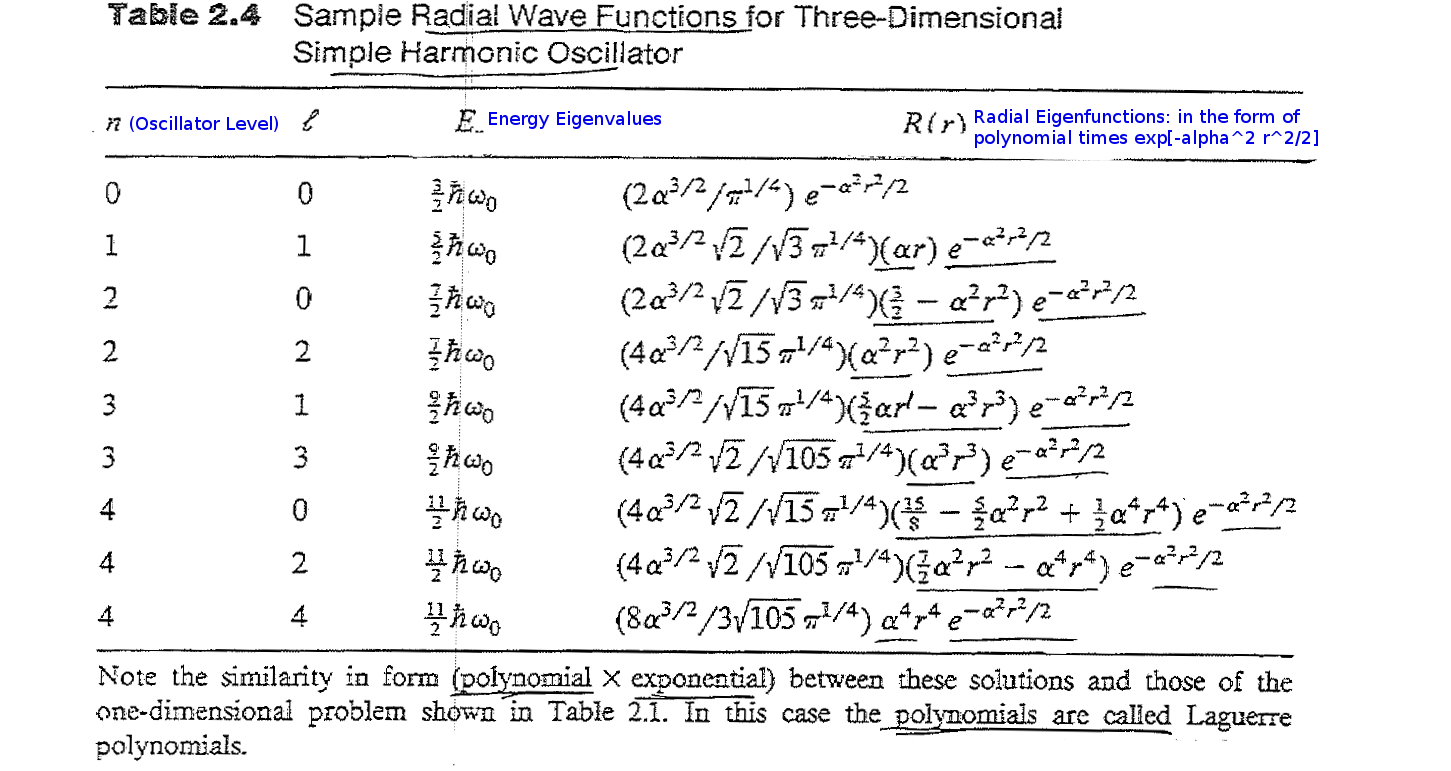
\includegraphics[width=6in]{images/shell/radial-wavefunction-SHO.png}
    \caption{Sample Radial Wave Functions for 3D Simple Harmonic Oscillator (Table 2.4, Krane)}
    \label{radial-wavefunction-SHO}
\end{table}

Harmonic Oscillator Energy Eigenvalues \footnote{See Liboff for details. $\frac{3}{2}$ is for 3D, it would be replaced by $\frac{1}{2}$ if we are discussing 1D}: 
\eqn{ E_n = \hbar \omega \left( n + \frac{3}{2} \right) - V_0^{\prime}  }
It is important to notice that energy does not depend on $l, m_l$, and not all values of $l$ are permitted for each $n$. From mathematical solution of the radial equation, the allowed quantum numbers: 
\begin{enumerate}
\item Given the Oscillator Level $n$, $l$ has to satisfy:
\eqn{ l \le n, \mbox{if n is even, then l has to be even; n is odd, l has to be odd.} }
\item Knowing $l$, $-l \le m_l \le l$, hence $2l+1$ degeneracy, also take into account $m_s = \pm \frac{1}{2}$, then the total degeneracy is \eqn{ D_l (l) = 2l+1, \fsp D_{l,s} (l) = 2(2l+1) = 4l+2 }
\item Written $D_{l,s}$ as a function of $n$, the total number of degeneracy is: 
\eqn{ D_l (n) = \frac{1}{2} (n+1)(n+2), \fsp D_{l,s} (n) = (n+1)(n+2) }
\end{enumerate}

Example: given $n =5$, $l = 1,3,5$. Then $ m_l = \pm 1, 0 (3); \pm 3, \pm 2, \pm 1, 0 (7); \pm 5, \pm 4, \pm 3, \pm 2, \pm 1, 0 (11)$. Together that is 21 degeneracy. Also take into account the 2 degeneracy of $m_s$, then in total there is 42 degeneracy. Notice this agrees with $D_n = (n+1)(n+2) = 42$. Table~\ref{energy-SHO} lists some lower energy levels \footnote{Spectroscopic Notation: $l=0 (s), l=1 (p), l=2 (d), l=3 (f), l=4 (g), l=5(h), l=6 (i), l=7(k), l=8(l), \cdots$. The letter is only associated with $l$ value, and the number distinguish this $(n,l)$ combination with a previous one}:  
\begin{table}[h!]
    \centering
    \begin{tabular}{|c|c|c|c|c|c|} \hline
    n & Energy $\frac{V_0 + E }{\hbar \omega_0}$ & states $(n,l)$ & Spectroscopic Notation & $D_{l,s} (n)$  & Cumulation $ \left( \Sum_n D_n \right)$ \\ \hline 
    0 & $3/2$ & (0,0) & 1s & 2 & 2 \\ \hline
    1 & $5/2$ & (1,1) & 1p & 6 & 8\\ \hline
    2 & $7/2$ & (2,0), (2,2) & 2s, 1d & 12 & 20 \\ \hline
    3 & $9/2$ & (3,1), (3,3) & 2p, 1f & 20 & 40 \\ \hline
    4 & $11/2$ & (4,0), (4,2), (4,4) & 3s, 2d, 1f & 30 & 70 \\ \hline
    \end{tabular}
    \caption{Lower Energy Levels of A Particle in a Central 3D Simple Harmonic Oscillator}
    \label{energy-SHO}
\end{table} 

Two issues with the harmonic oscillator model:  
\begin{enumerate}
\item The total number of allowed energies are correct for $n = 0,1,2$, but off for higher magic numbers.  
\item The separation energy:  
\eqn{ \Delta E = \hbar \omega \left[ \left( n + 1 + \frac{3}{2} \right) - \left( n + \frac{3}{2} \right) \right] = \hbar \omega = \hbar \sqrt{\frac{2V_0}{m R_0^2} - \frac{(Z-1) e^2}{R_0^3} }  }
For neutrons, if we plug in $R_0 = 1.25 A^{1/3} \fsp \fm$, and get ride of the coulomb term, then $V_0 \approx 50 A^{-1/3} \MeV$. We notice as A increases, $\Delta E $ approaches 10 MeV. That is to say, for a typical well depth of 50 MeV, we can fit around 4 oscillator energy levels in it, which does not agree with reality\footnote{there are clearly A's that have more than 4 possible energy levels.}. Notice the above discussion is for neutrons. The energy levels are shifted up for protons. 
\end{enumerate}



%%%%%%%%%%%%%%%% Intermediate Potentials %%%%%%%%%%%%%
\topic{Intermediate Potential}
\begin{figure}[h!]
    \centering
    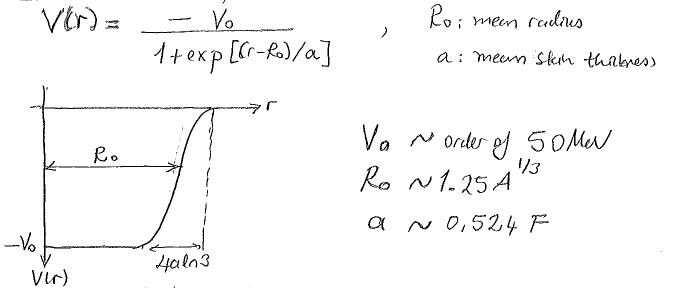
\includegraphics[width=4in]{images/shell/intermediate-form-potential.png}
    \caption{Intermediate Form Potential Diagram}
\end{figure}

It is more representative of strong potential, with sufficiently sharp edge, and sufficiently smooth decay to reach zero around $R_0$. As seen in Figure~\ref{intermediate-energy}, again magical number 2,8, 20 are predicted correctly, but higher shell occupancy numbers are off. 

\begin{figure}[h!]
    \centering
    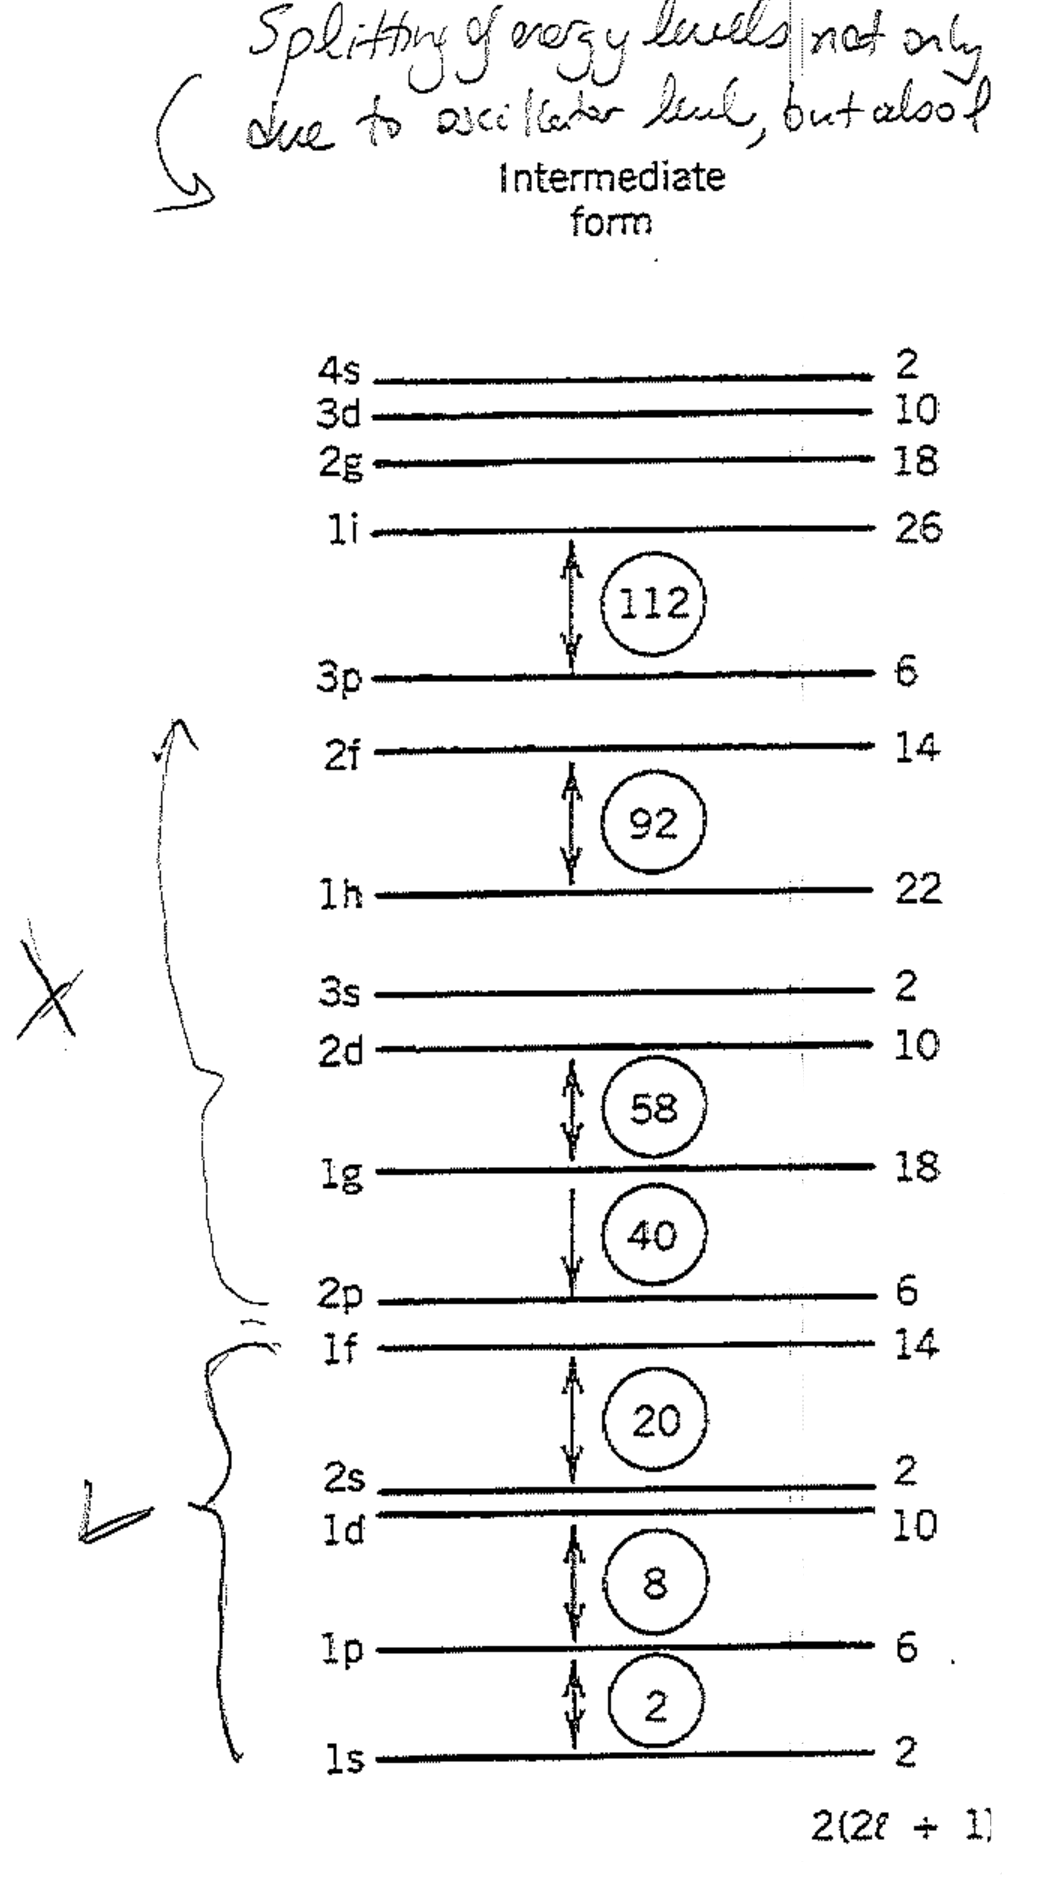
\includegraphics[width=2in]{images/shell/intermediate-potential-energy.png}
    \caption{Intermediate Form Energy Level Diagram, Krane Figure 5,6 (a)}
    \label{intermediate-energy}
\end{figure}



%%%%%%%%%%%%%%%% Spin-orbit Coupling %%%%%%%%%%%%%
\topic{Spin-Orbit Coupling}
\subtopic{Potential with Spin-Orbit Coupling}
Our previous attempts suggest that single particle interaction is missing something fundamental. Thus we add the interaction between the orbital angular momentum and the intrinsic spin angular momentum of nucleon: 
\eqn{ V_{\mathrm{nuc}} (r) = V_0 (r) + V_{\mathrm{so}} (r) \frac{\lhat \cdot \shat}{\hbar^2} }
Notice:
\begin{itemize}
\item $\lhat, \shat$ are operators on a single nucleon; 
\item the $\frac{\lhat \cdot \shat}{\hbar^2}$ term could give the proper separation of the sub-shells;
\item Adding spin-orbit coupling does not destroy the physical content of the potential as the intermediate potential is a good guess for how the nuclear potential should look like; 
\item \textcolor{blue}{the interaction is NOT spherically symmetric.}
\end{itemize} 

\begin{align}
\expect{\lhat \cdot \shat} &= \frac{\hbar^2}{2} \left[ j(j+1) - l(l+1) - \frac{3}{4} \right] =
\begin{dcases*}
- \frac{\hbar^2}{2} (l+1) & for $j = l-\frac{1}{2}$. \\ 
\frac{\hbar^2}{2} l & for $j = l + \frac{2}{2}$. 
\end{dcases*} 
\\
V_{\mathrm{nuc}} (r) &= 
\begin{dcases*}
V_0 - \frac{l+1}{2} V_{\mathrm{so}} & for $j = l-\frac{1}{2}$. \\ 
V_0 + \frac{l}{2} V_{\mathrm{so}} & for $j = l + \frac{2}{2}$. \\
\end{dcases*}
\end{align}
Keep in mind that $V_0 < 0, V_{\mathrm{so}} < 0$, so 
\begin{itemize}
\item $j = l+\frac{1}{2}$: pushes the well and the energy levels down (lower), more tightly bound; the attractive well is more attractive; 
\item $j = l - \frac{1}{2}$: pushes the well and the energy levels higher (up), more weakly bound.  
\end{itemize}

\subtopic{Consequences of Spin-orbit Coupling}
\begin{enumerate}
\item Each of the original $l$ level would be spitted into two states $j= l \pm \frac{1}{2}$ as in Figure~\ref{s-o-coupling}. Notice the total number of states preserved even though degeneracy is not based on $m_l, m_s$ in this new notation. We use spectroscopic notation $nl_j$.  
\begin{figure}[h!]
    \centering
    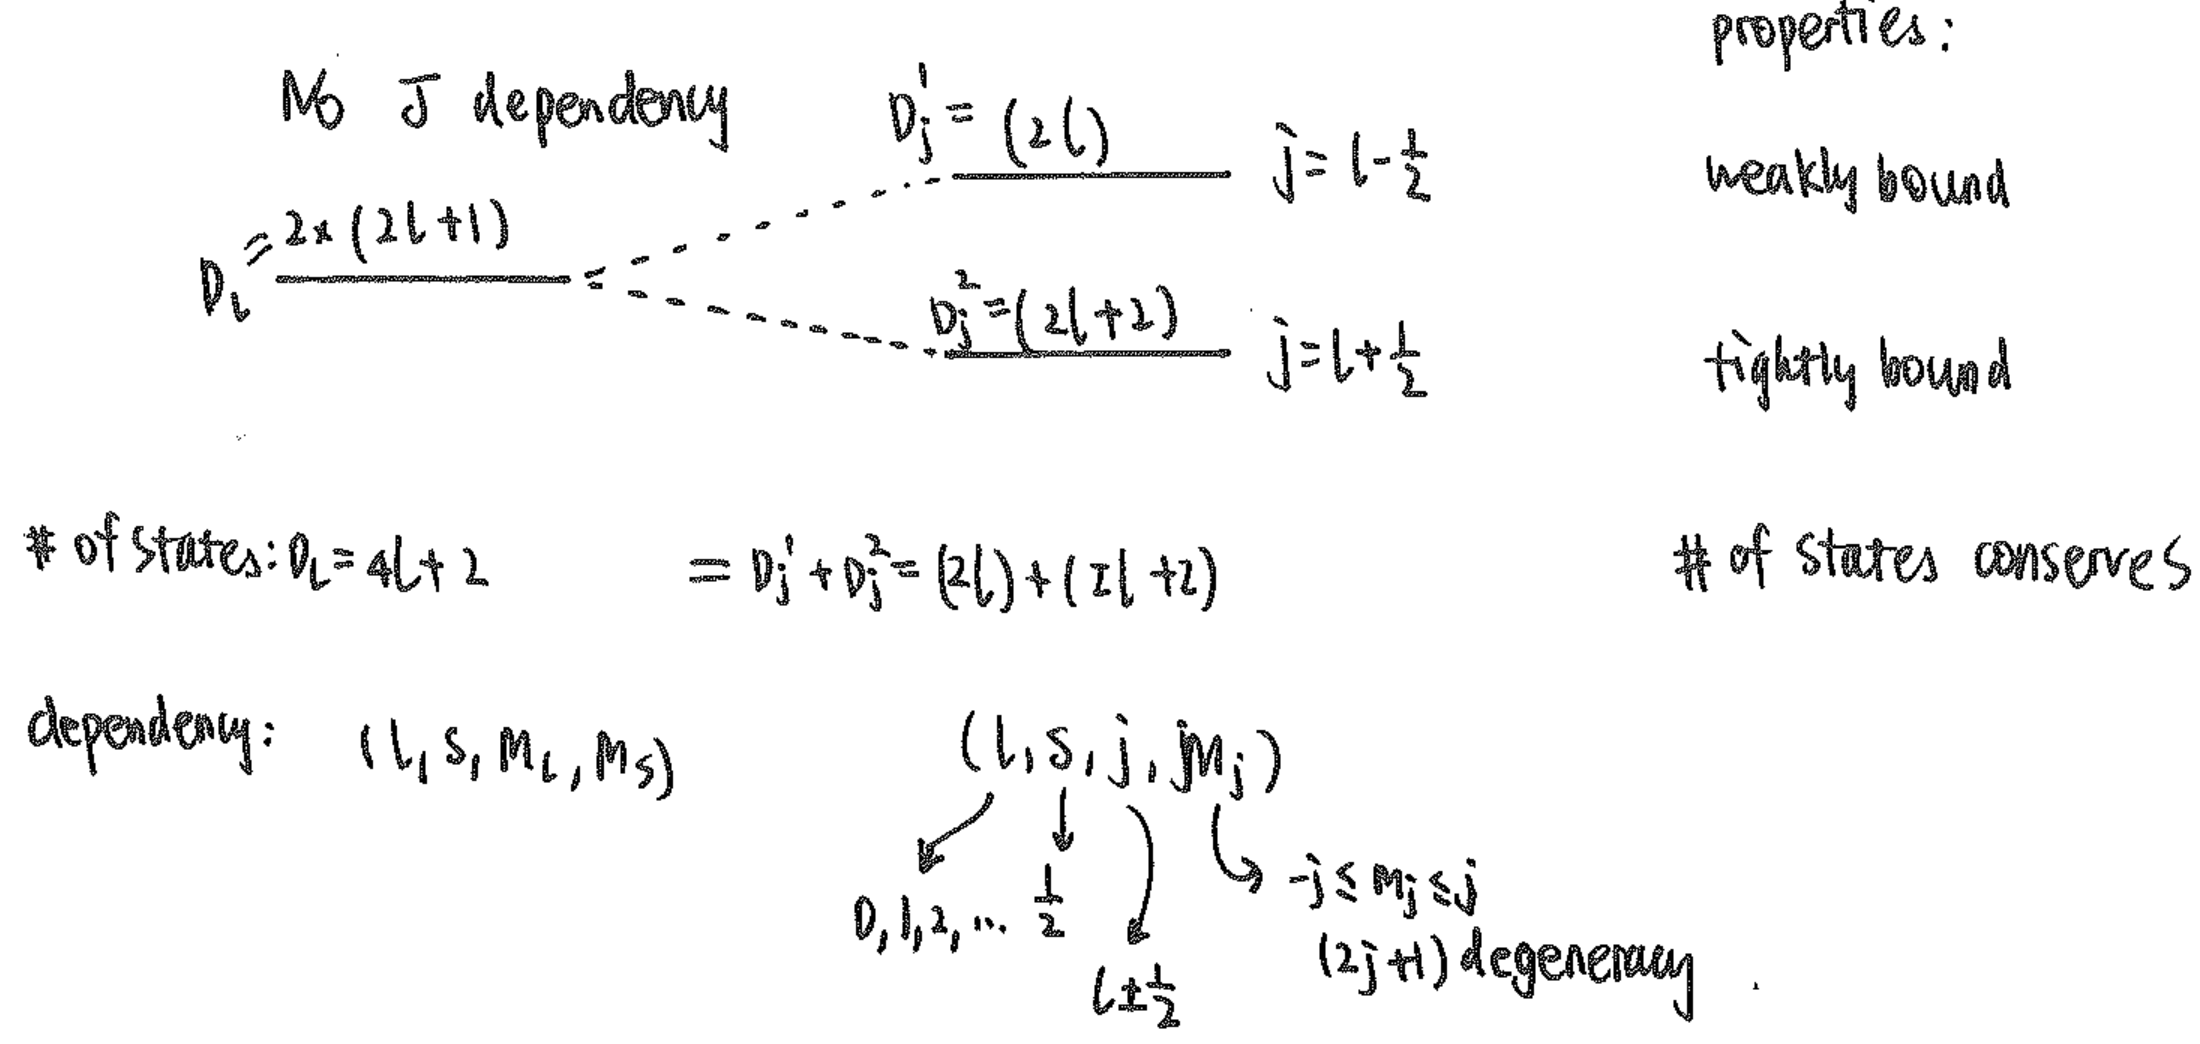
\includegraphics[width=4.6in]{images/shell/spin-orbit-coupling.png}
    \caption{Spin-Orbit Coupling, Splitting the Original $l$ Level into Two States}
    \label{s-o-coupling}
\end{figure}

\item The $j=l-\frac{1}{2}$ state makes the well shallower, making the state more weakly bound; the $j=l+\frac{1}{2}$ staet makes the well deeper, making the state more tightly bound. 
\begin{figure}[h!]
    \centering
    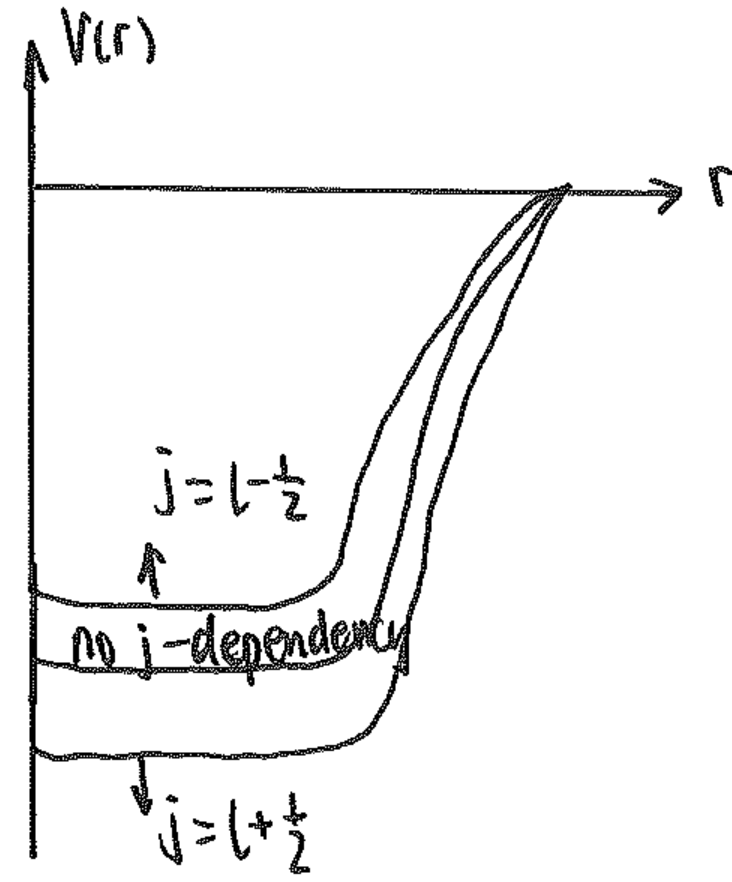
\includegraphics[width=1.5in]{images/shell/spin-orbit-coupling-potential.png}
    \caption{Potential Shifts after Applying Spin-Orbit Coupling}
\end{figure}

\item For a pair of states with $l>0$, the energy splitting difference increases with increasing $l$:
\eqn{ \Delta E = \expect{ \lhat \cdot \shat }_{j = l+\frac{1}{2} } - \expect{ \lhat \cdot \shat }_{j = l-\frac{1}{2} } = \frac{\hbar^2}{2} (2l+1) }
The physical interpretation of the this is that states with larger $l$ values split more; for instance, $1f$ state split more than than $2p$. In the deuteron example, $l=0$, hence we do not consider spin-orbit coupling. 
\end{enumerate}


\subtopic{Correction to the Intermediate Form Potential Shell Model}
\textcolor{blue}{Splitting of highest $l$ (recall larger $l$ results in larger $\Delta E$) at each oscillator level leads to re-joining of new j-levels with the top of the lower shell, and accounts for all the magic numbers.} Even the non-existing 184 is predicted. This founding leads to a Nobel Prize. 
\begin{enumerate}
\item $n=3$ oscillator level, the induced $1f_{7/2}$ reduces 8 nucleons from the upper shell, and makes a new `intermediate' shell with 8 nucleons ($D(1f_{7/2}) = 2\times j + 1 = 8$), which account for the magic number of 28 (=20+8). See Figure~\ref{shell-28}.
\begin{figure}
    \centering
    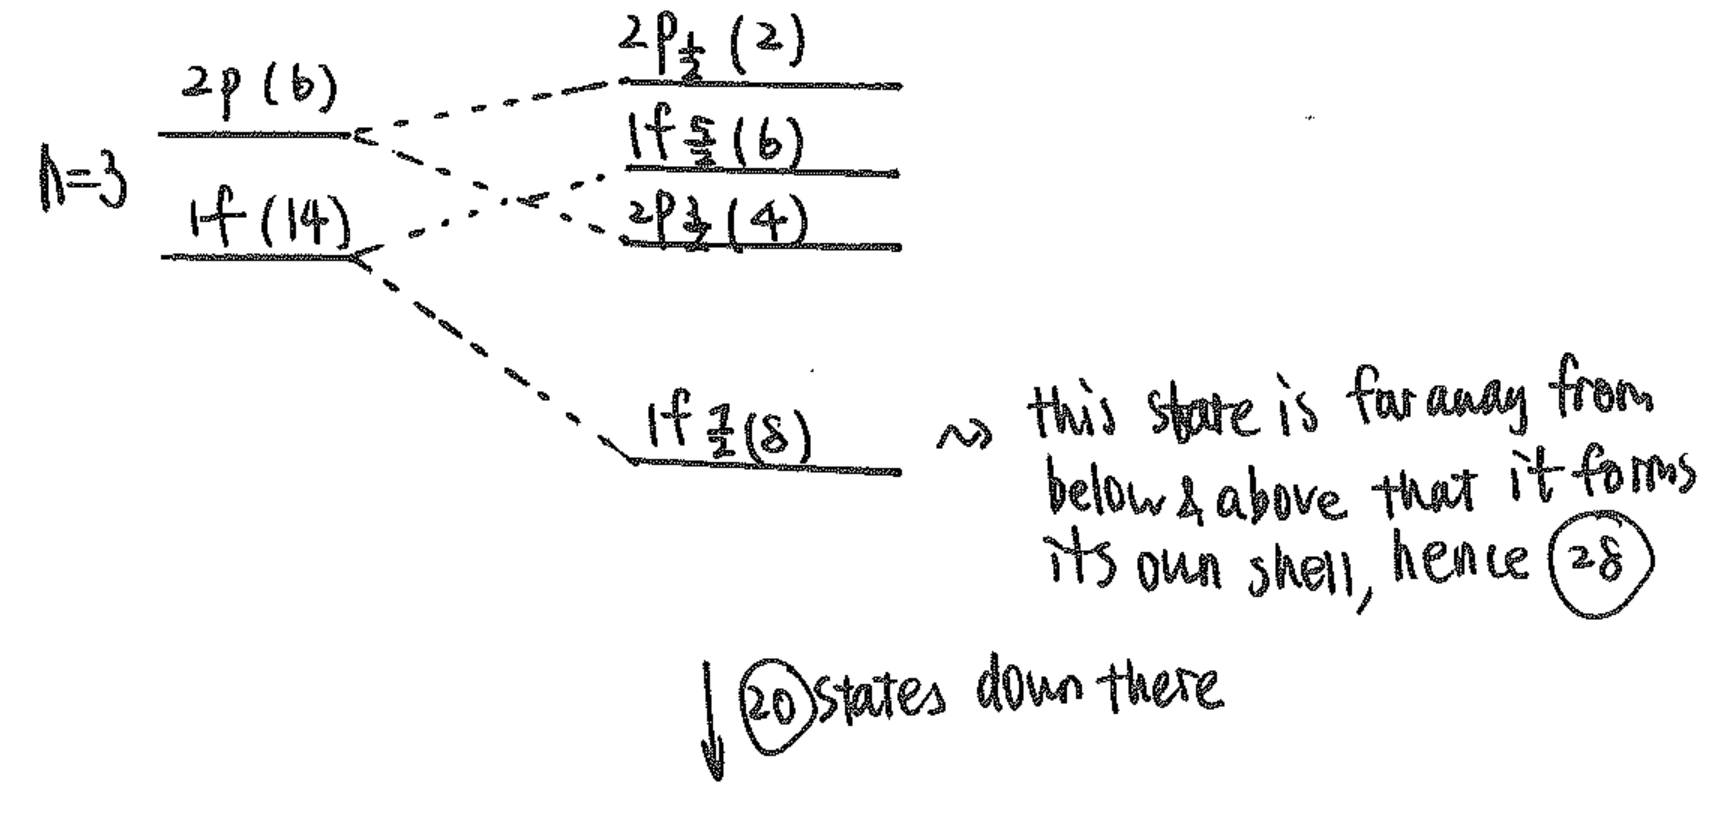
\includegraphics[width=3.5in]{images/shell/magic-number-28.png}
    \caption{Correction to Shell Model $n=3$\label{shell-28}}
\end{figure}

\item $n=4$ oscillator level: Figure~\ref{shell-50}.
\begin{figure}
    \centering
    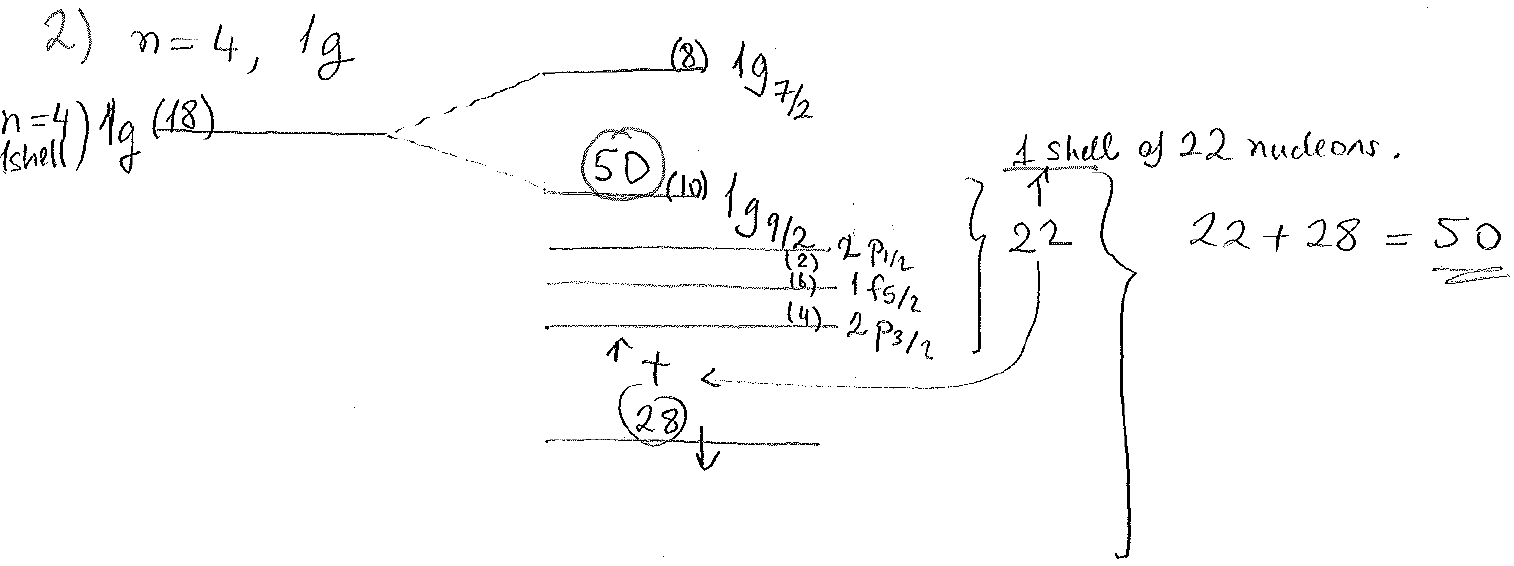
\includegraphics[width=4in]{images/shell/magic-number-50.png}
    \caption{Correction to Shell Model $n=4$\label{shell-50}}
\end{figure}

\item $n=5$ oscillator level: Figure~\ref{shell-82}.
\begin{figure}
    \centering
    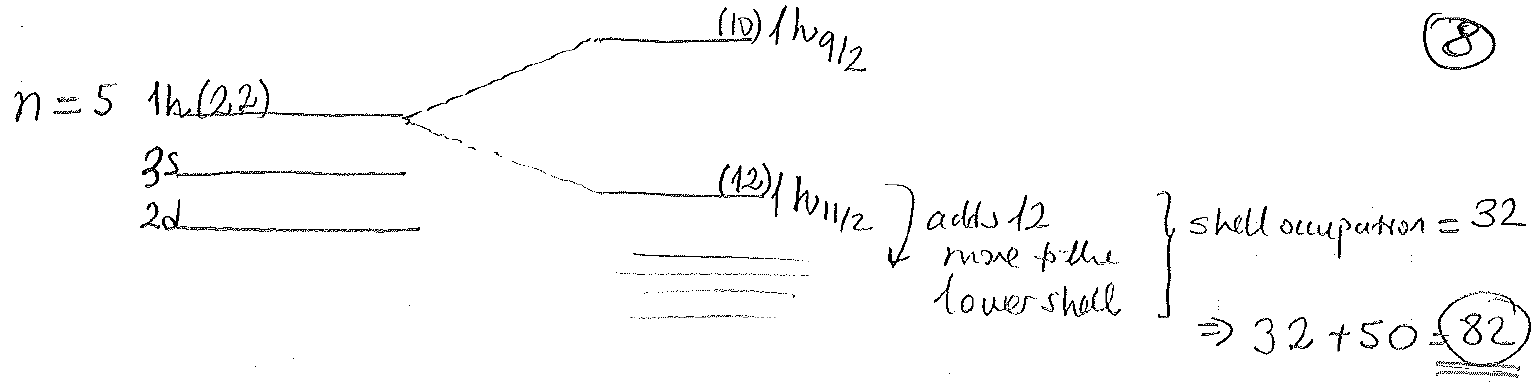
\includegraphics[width=4in]{images/shell/magic-number-82.png}
    \caption{Correction to Shell Model $n=5$\label{shell-82}}
\end{figure}

\item $n=7$ oscillator level: Figure~\ref{shell-126}.
\begin{figure}
    \centering
    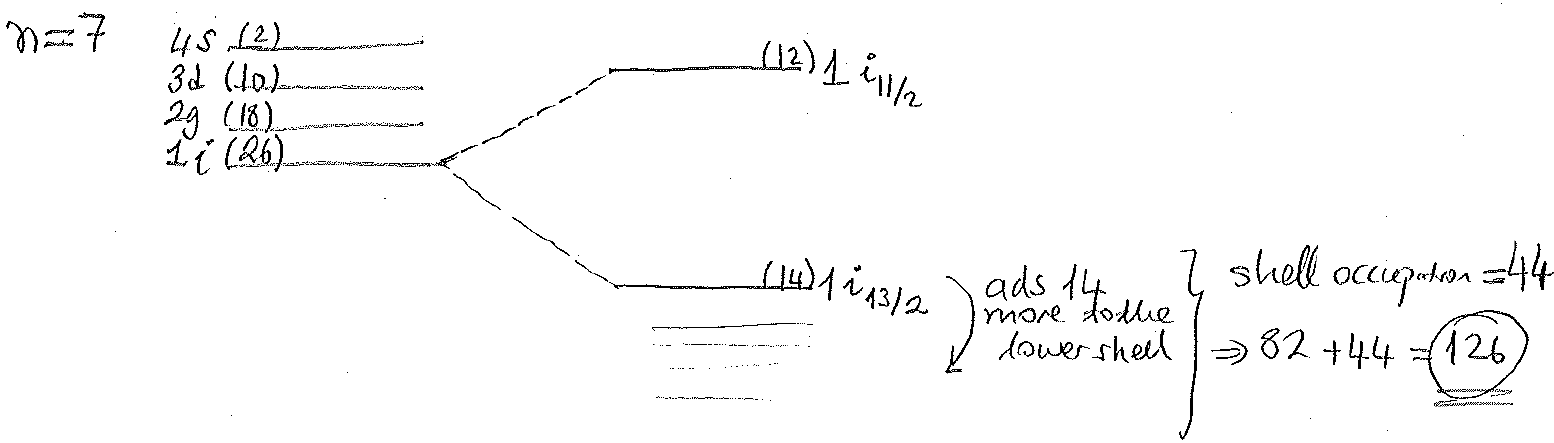
\includegraphics[width=4in]{images/shell/magic-number-126.png}
    \caption{Correction to Shell Model $n=7$\label{shell-126}}
\end{figure}
\end{enumerate}

\uline{Summary}
\begin{enumerate}
\item Know what $l$ values each letter correspond to: $ f \to l=3, g \to l=4$ (starting from $l=0$, the notation goes like: s, p, d, f, h, g). 
\item After knowing $l$, the newly split states are $j= l \pm \frac{1}{2}$, write the new states out as original notation$_{j}$;
\item Degeneracy:$2 j+1$ degeneracy.  
\end{enumerate}



\end{document}
